
\chapter{KDEs, JSON}
\label{ch:KDEs}

\section{Kernel Density Estimates (KDEs)}

\subsection{Limitations of histograms}

Histograms are a great tool for seeing the distribution of a numerical,
univariate sample. One problem with them, though, is that a data set doesn't
uniquely determine a histogram: instead, we must specify parameters such as
the bin size and the ``alignment'' of the bins (\textit{i.e.}, where exactly
the breaks occur), and the resulting display is colored by those choices.

Consider this simple data set (from Janert, 2010):

\begin{center}
\texttt{2.1, 2.3, 1.9, 1.8, 1.4, 2.6, 1.7, 2.2}
\end{center}

Suppose we choose a bin width of 1. If we positioned the \textit{left} edge of
each bin at 0, 1, 2, 3, ..., we would get the histogram on the left side of
Figure~\ref{fig:histBinParadox}.

\begin{Verbatim}[fontsize=\footnotesize,samepage=true,frame=single]
data = np.array([2.1, 2.3, 1.9, 1.8, 1.4, 2.6, 1.7, 2.2])
plt.hist(data, bins=[0,1,2,3,4])
\end{Verbatim}

Our interpretation would probably be: ``looks like the values occur pretty
uniformly throughout the range 1-3.''

But if we shifted our bin alignment to be on the ``halves'' (0.5, 1.5, 2.5,
...), we get this histogram on the \textit{right} side of
Figure~\ref{fig:histBinParadox}.

\begin{Verbatim}[fontsize=\footnotesize,samepage=true,frame=single]
plt.hist(data, bins=[-.5,0.5,1.5,2.5,3.5,4.5])
\end{Verbatim}

Now we may be liable to think: ``it looks like a steeply-peaked distribution
with most values right near the center value of 2.''

\smallskip
Yet the data is the \textit{same}!
\smallskip

\begin{figure}[ht]
\centering
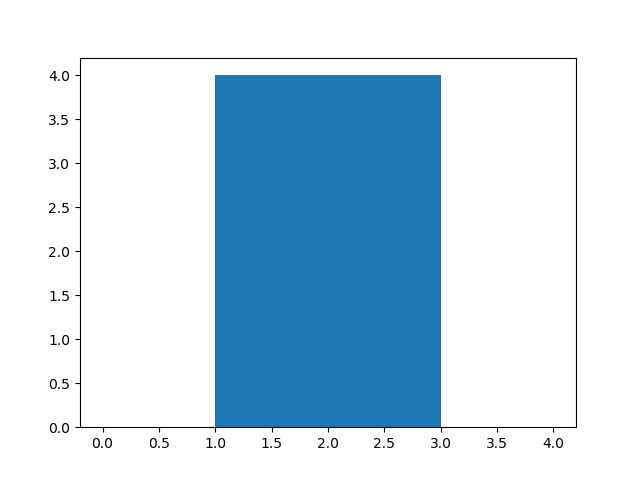
\includegraphics[width=0.45\textwidth]{hist1.png}
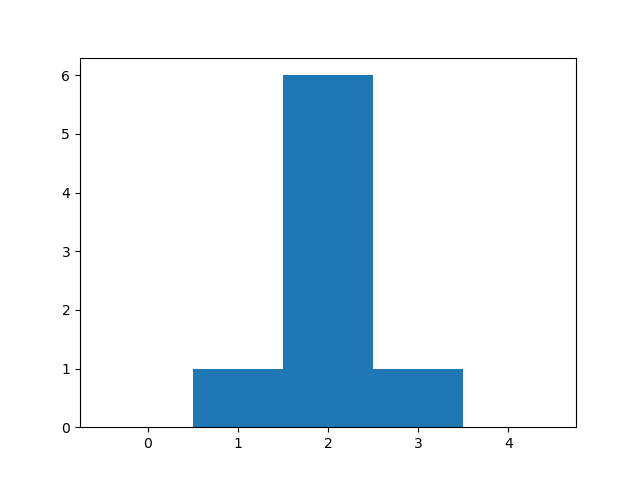
\includegraphics[width=0.45\textwidth]{hist2.png}
\caption{Two histograms of the \textit{same} data set!}
\label{fig:histBinParadox}
\end{figure}
\begin{center}
\end{center}



Histograms have a couple other problems as well:

\begin{itemize}
\itemsep.1em
\item They inherently lose information, since by definition data points with
specific, precise values are munged into ``the nearest bin.''
\item They don't handle outliers very well. A single outlier way outside the
normal range forces us to either (a) include a lot of empty cells in the
middle, or (b) choose an unreasonably wide bin width that doesn't work for the
majority of points.
\end{itemize}

One solution to these problems is a more advanced technique called
\textit{Kernel Density Estimates.}

\subsection{Kernels}

A ``kernel'' is defined as a single, strongly-peaked function that has an area
under its curve of exactly 1. Normally (no pun intended!) we will use a
\textit{Gaussian kernel}, which means ``a bell curve a la the normal
distribution.'' 

One thing we have to decide is the \textit{width} of this kernel --- which in
our case essentially means ``the standard deviation of the normal
distribution we're using.'' This is kind of like having to choose the bin width
for histograms, but in practice it turns out not to 

To form a KDE, we place a ``copy'' of this kernel at each data point, and then
add up all the kernel contributions to make a smooth curve.

There are several different ways to do this with Python packages. The Seaborn
library has a good ``\texttt{kdeplot()}'' function. Using straight SciPy, we
can call the \texttt{gaussian\_kde()} function and pass it the bandwidth as a
second argument. This returns a function that can be used to evaluate the KDE
at any data point. (Read that sentence again: a function that returns a
function? It can be confusing.) Then, we can plot it by creating a range of
values to evaluate the KDE at, and plotting those values against the KDE's
values.

It's easier than it sounds when you run the actual code:

\begin{Verbatim}[fontsize=\footnotesize,samepage=true,frame=single]
import scipy.stats
kde = scipy.stats.gaussian_kde(data,bw_method=2)
x_vals = np.arange(0,4,.1)
plt.plot(x_vals,kde(x_vals))
\end{Verbatim}

Choosing a larger kernel width effectively smooths out the KDE more, making
each point ``fuzzier'' with respect to its actual position. Choosing a narrower
kernel focuses each data point's contribution more at its actual value,
making the plot choppier.

\begin{figure}[ht]
\centering
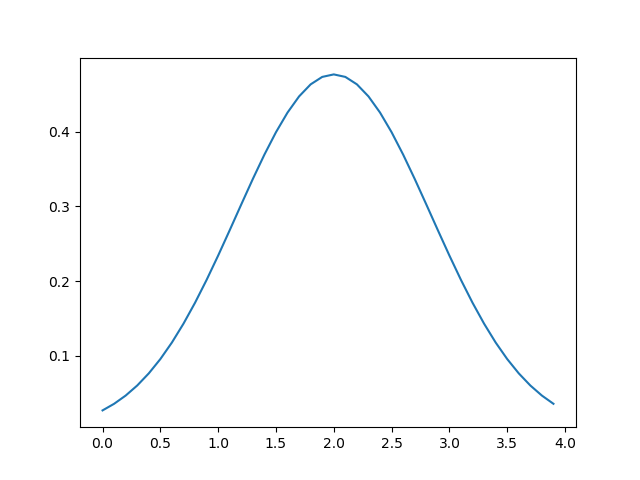
\includegraphics[width=0.4\textwidth]{kde1.png}
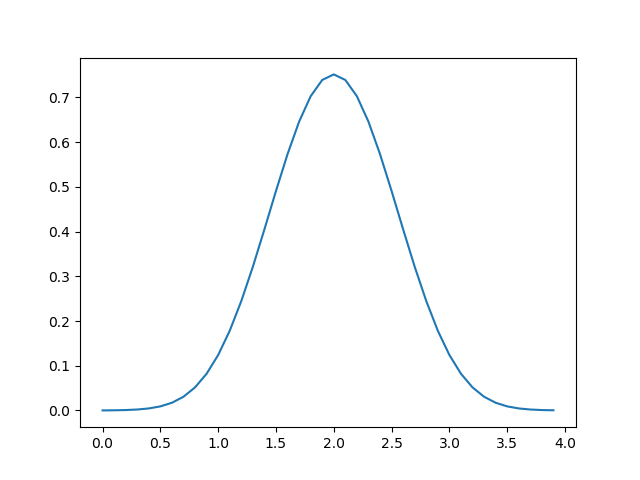
\includegraphics[width=0.4\textwidth]{kde2.png}
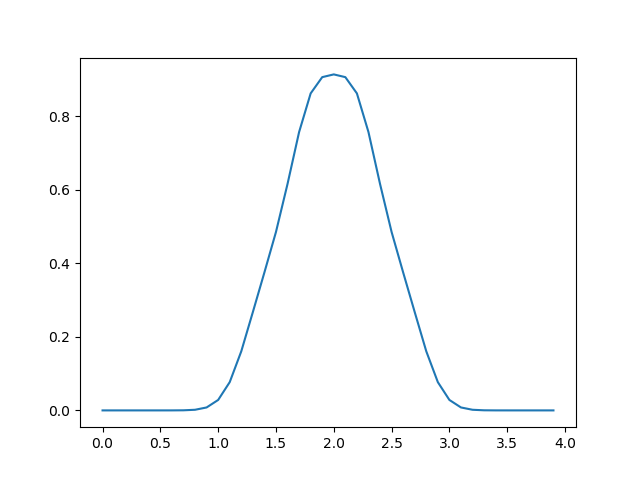
\includegraphics[width=0.4\textwidth]{kde3.png}
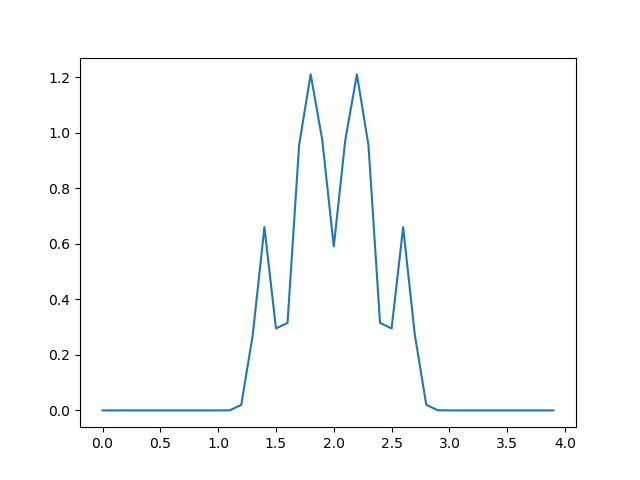
\includegraphics[width=0.4\textwidth]{kde4.png}
\caption{Gaussian KDEs with bandwidths of 2, 1, .5, and .2, respectively.}
\end{figure}

In practice, it's another parameter to play with. If the data follows a smooth
distribution, you can use a wider bandwidth which will ``blur'' each data point
more and give a more intuitive view of the general distribution
characteristics. If the distribution is more ``wiggly,'' though, you need a
narrower bandwidth to see all the relevant detail.

Like most things in Data Science (and in life), there's no one true
hard-and-fast right answer. There is instead a range of points of view, many
of which may be illuminating.


\section{JSON}

JSON (pronounced like the name ``Jason'') is a simple, human-readable text file
format that is very commonly used for information storage and interchange. (It
stands for ``JavaScript Object Notation,'' but don't be fooled: it doesn't have
much to do with the JavaScript language except historically. \textit{Any}
language, including Python, can read/write JSON data.)

The really nice things are (1) it's simple, and easy on the eyes (unlike
binary formats, or XML), and (2) it structures information hierarchically in
list-ish, dictionary-ish, string-ish type elements that will be instantly
familiar to you. A JSON ``document'' is, in fact, \textit{essentially a Python
list or dictionary with embedded contents.}

Here's an example file in JSON format:

\small
\begin{Verbatim}[fontsize=\small,samepage=true,frame=none]
{"name": "Luke Skywalker", "rank": "Jedi", "lightsaber color": "blue",
"episodes": ["IV", "V", "VI", "VII", "VIII"], "relations": {"Leia": "sister",
"Han": "friend", "Artoo": "servant", "Rey": "student"}}
\end{Verbatim}
\normalsize

Its structure is instantly apparent: a dictionary whose values are strings,
lists, and other dictionaries, as appropriate.

Probably the best thing about JSON is that once we read and parse a JSON file
or other information source, we have a bona fide Python object that we can
treat in the ordinary way.

In Python, we have the \texttt{json} package, which you can import like any
other:

\begin{Verbatim}[fontsize=\small,samepage=true,frame=single]
    import json
\end{Verbatim}

There are four functions that matter:
\small
\begin{compactitem}
\item \texttt{json.dump}(\textit{someObject}, \textit{aFile}) - Dump the Python
object to a file in JSON text format.
\item \texttt{json.dumps}(\textit{someObject}) - Dump the Python
object to a string in JSON text format (and return it).
\item \texttt{json.load}(\textit{aFile}) - Build and return a Python
object from the contents of the JSON text file.
\item \texttt{json.loads}(\textit{someString}) - Build and return a Python object
from the JSON text string.
\end{compactitem}

\normalsize
So, for instance, to load a file \texttt{info.json} into a Python object
called ``\texttt{my\_stuff}'':

\small
\begin{Verbatim}[fontsize=\small,samepage=true,frame=single]
    with open('info.json','r') as f:
        my_stuff = json.load(f)
\end{Verbatim}

\normalsize
We could parse and access the Luke Skywalker file just like this:

\small
\begin{Verbatim}[fontsize=\small,samepage=true,frame=single]
    with open('luke.json','r') as f:
        luke = json.load(f)
    print(luke['lightsaber color'])
    blue

    print(luke['episodes'][2])
    VI
\end{Verbatim}

\normalsize
Simple as that!

\section{``Hierarchical'' vs. ``flat'' data}

You can see that the JSON file format is essentially a textual representation
of an arbitrarily nested Python object. This object can be a list or a
dictionary, and have embedded lists and dictionaries to any arbitrary level of
nesting. Here's another example:

\begin{Verbatim}[fontsize=\small,samepage=true,frame=none]
[{"prefix": "DATA", "num": 219, "creds": 3, "instructor": "Davies",
"meetings": [{"time": {"day": "TR", "time": "2pm"}, "location": {"bldg":
"Trinkle", "room": "B6"}}], "roster": [{"first": "Lady", "last": "Gaga",
"email": "lgaga@umw.edu"}, {"first": "The", "last": "Rock", "email":
"trock@umw.edu"}, ...
\end{Verbatim}

When you disentangle this, you'll realize that what you have is:

\vspace{.2in}

\large
\noindent A list, each element of which is:\\
$\bullet$ a dictionary, with key/value pairs:
        \begin{compactenum}
        \item \texttt{prefix}: a string
        \item \texttt{num}: an int
        \item \texttt{creds}: an int
        \item \texttt{instructor}: a string
        \item \texttt{meetings}: a list, each element of which is:
            \begin{compactitem}
            \item a dictionary, with key/value pairs:
                \begin{compactenum}
                \item \texttt{time}: a dictionary, with key/value pairs:
                    \begin{compactenum}
                    \item \texttt{day}: a string
                    \item \texttt{time}: a string
                    \end{compactenum}
                \item \texttt{location}: a dictionary, with key/value pairs:
                    \begin{compactenum}
                    \item \texttt{bldg}: a string
                    \item \texttt{room}: a string
                    \end{compactenum}
                \end{compactenum}
            \end{compactitem}
        \item \texttt{roster}: a list, each element of which is:
            \begin{compactitem}
            \item a dictionary, with key/value pairs:
                \begin{compactenum}
                \item \texttt{first}: a string
                \item \texttt{last}: a string
                \item \texttt{email}: a string
                \end{compactenum}
            \end{compactitem}
        \item ...and possibly other stuff...
        \end{compactenum}

\normalsize

\pagebreak

This kind of structure is called \textbf{hierarchical} data. This is in
contrast to so-called \textbf{flat} data, like a CSV:

\begin{Verbatim}[fontsize=\small,samepage=true,frame=none]
Prefix,Num,Instructor,Creds,Bldg,Room,Day,Time
DATA,219,Davies,3,Trinkle,B6,TR,2pm
ENGL,286,Rigsby,3,Combs,112,MWF,11am
CPSC,305,Finlayson,4,Trinkle,B52,MWF,8am
\end{Verbatim}

It should be clear that hierarchical data is intrinsically \textit{more
expressive} than flat data. Rather than each data record being a strict,
identical-length sequence of values, the whole nested structure communicates
order and relationships between subcomponents, like an outline.

It's not even always possible, let alone straightforward, to convert from a
hierarchical format to a flat format. Consider the JSON file above: it permits
any number of \texttt{meetings} for a single course, each of which has
embedded structure. In this case, the structure for each meeting is regular,
since it's apparently composed of a fixed number of fields with unique names.
(This won't always be the case, and if it's not, we would \textit{lose
information} in collapsing it to a flat format.) Even so, though, it's not
clear what to do with the multiple meeting times/locations for a course. Do we
make each \texttt{Bldg/Room/Day/Time} group into its own set of headings in
the flat format? This brings with it its own problems, such as:

\begin{compactenum}
\item How do we associate each group of buildings/rooms/days/times together,
since they're now all individual top-level fields? (Naming conventions seem
like the only solution, and it's awkward.)
\item How do we know the maximum number of such meetings, so as to specify the
width of the table?
\item What do we do for rows which don't have the maximum number of meetings?
Leave the others blank?
\item How do we perform standard queries like ``find all courses that have at
least one meeting in Trinkle?'' (We have to split this up into an awkward query
that separately queries each of the columns and unions the answer.)
\end{compactenum}

There are better ways to organize such data, such as the \textbf{relational
model} that has been ubiquitous in database schema design since Ted Codd
invented it in the 1960's. It allows us to ``normalize'' such data sets and
represent them in multiple, interrelated tables. We'll take a look at this
when we look at SQLite later in the course. Some irregular structures defy
even the relational model, however, which is why some newer database paradigms
(like NoSQL databases) have been developed to get around its limitations.

One big reality to grasp, however, is that at this point in time,
\textit{almost all machine learning algorithms are based on a \textbf{flat}
data structure}. There are some quite advanced, cutting-edge exceptions to
this, but really the field of mining hierarchical (and other non-flat) data
formats is still in its infancy. Lots of opportunity to make a name for
yourself here!
